Noticing if assumptions are not met is important when looking at data from real life.
To understand how breached assumptions look when modeled, looking at realistic data becomes necessary. \newline

\begin{figure}[h!]
	\centering
	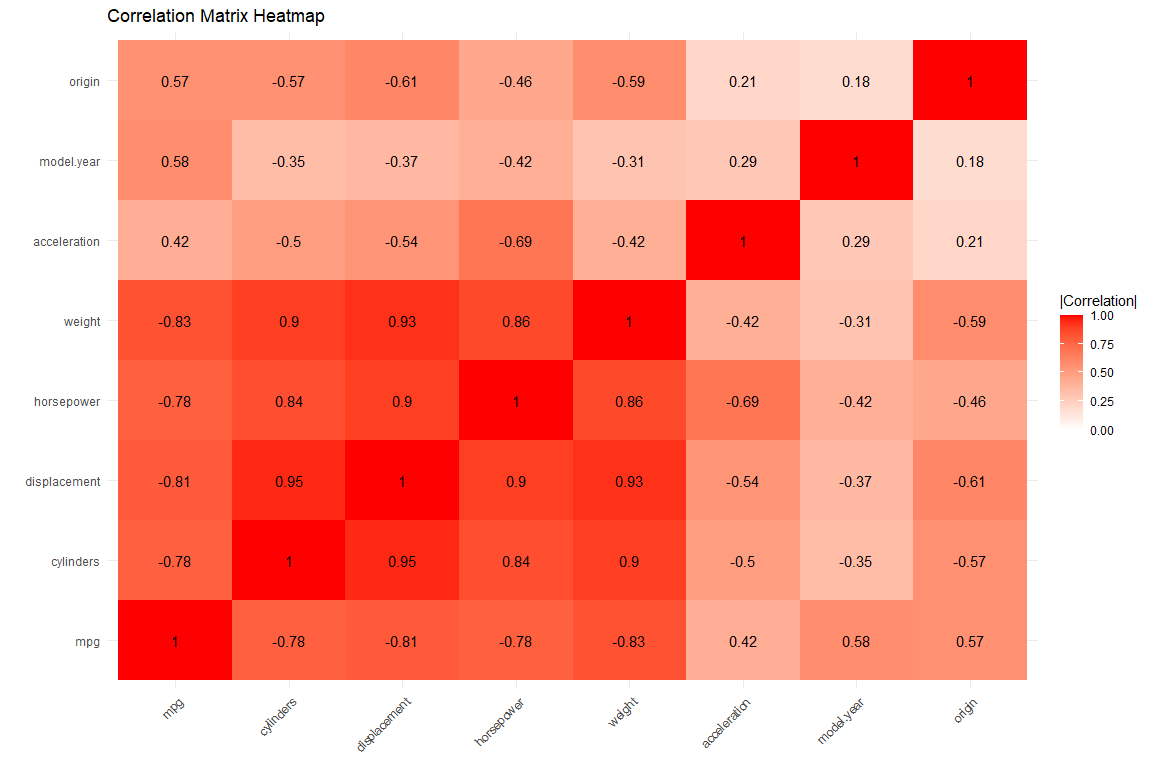
\includegraphics[width=\linewidth]{billder/1.png}
	\caption{HER}
	\label{fig:HEAT}
\end{figure}
Multicollinearity can be seen in figure 1 this heatmap made from the MPG dataset. Multicollinearit occurs when independent variables are highly correlated with each other, and as a result, it becomes more difficult to isolate the individual effect of each variable in a regression model.
In this model it is shown through the numbers, where the high numbers suggest a strong linear relationship through the variables. So between 'displacement' and ' cylinders', the value is 0.95, which is close to 1 and therefore shows there is multicollinearity. \newline

\begin{figure}[h!]
	\centering
	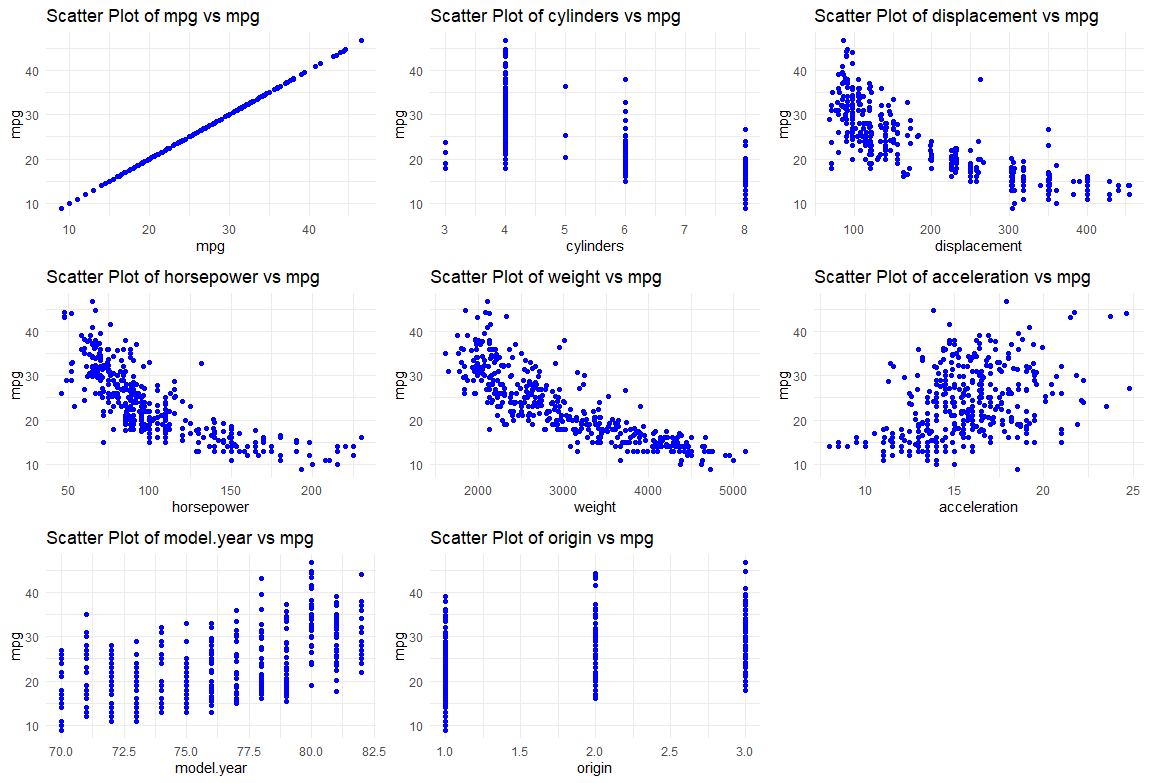
\includegraphics[width=\linewidth]{billder/2.png}
	\caption{HER}
	\label{fig:Scatter}
\end{figure}
in figure 2 is an example of hetereoscedasticity in the 'mpg' and 'horsepower' scatterplot, where there is not constant variance of the residuals. This is seen because there is a big spread between the variables, especially when horsepower decreases.   